\documentclass{extbook}[14pt]
\usepackage{multicol, enumerate, enumitem, hyperref, color, soul, setspace, parskip, fancyhdr, amssymb, amsthm, amsmath, bbm, latexsym, units, mathtools}
\everymath{\displaystyle}
\usepackage[headsep=0.5cm,headheight=0cm, left=1 in,right= 1 in,top= 1 in,bottom= 1 in]{geometry}
\usepackage{dashrule}  % Package to use the command below to create lines between items
\newcommand{\litem}[1]{\item #1

\rule{\textwidth}{0.4pt}}
\pagestyle{fancy}
\lhead{}
\chead{Answer Key for Progress Quiz 4 Version A}
\rhead{}
\lfoot{9187-5854}
\cfoot{}
\rfoot{Spring 2021}
\begin{document}
\textbf{This key should allow you to understand why you choose the option you did (beyond just getting a question right or wrong). \href{https://xronos.clas.ufl.edu/mac1105spring2020/courseDescriptionAndMisc/Exams/LearningFromResults}{More instructions on how to use this key can be found here}.}

\textbf{If you have a suggestion to make the keys better, \href{https://forms.gle/CZkbZmPbC9XALEE88}{please fill out the short survey here}.}

\textit{Note: This key is auto-generated and may contain issues and/or errors. The keys are reviewed after each exam to ensure grading is done accurately. If there are issues (like duplicate options), they are noted in the offline gradebook. The keys are a work-in-progress to give students as many resources to improve as possible.}

\rule{\textwidth}{0.4pt}

\begin{enumerate}\litem{
Which of the following equations \textit{could} be of the graph presented below?

\begin{center}
    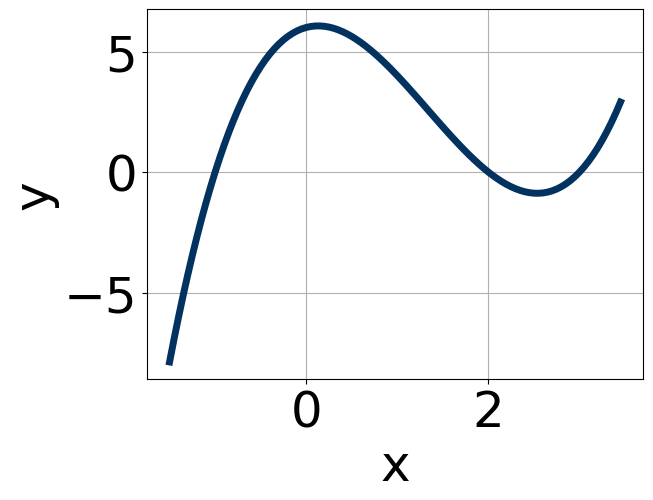
\includegraphics[width=0.5\textwidth]{../Figures/polyGraphToFunctionCopyA.png}
\end{center}


The solution is \( 3x^{10} (x - 3)^{10} (x - 1)^{7} \), which is option B.\begin{enumerate}[label=\Alph*.]
\item \( 12x^{5} (x - 3)^{6} (x - 1)^{8} \)

The factor $x$ should have an even power and the factor $(x - 1)$ should have an odd power.
\item \( 3x^{10} (x - 3)^{10} (x - 1)^{7} \)

* This is the correct option.
\item \( -16x^{6} (x - 3)^{6} (x - 1)^{6} \)

The factor $(x - 1)$ should have an odd power and the leading coefficient should be the opposite sign.
\item \( 10x^{7} (x - 3)^{8} (x - 1)^{9} \)

The factor $x$ should have an even power.
\item \( -4x^{4} (x - 3)^{6} (x - 1)^{9} \)

This corresponds to the leading coefficient being the opposite value than it should be.
\end{enumerate}

\textbf{General Comment:} General Comments: Draw the x-axis to determine which zeros are touching (and so have even multiplicity) or cross (and have odd multiplicity).
}
\litem{
Describe the end behavior of the polynomial below.
\[ f(x) = -8(x - 6)^{4}(x + 6)^{5}(x - 3)^{3}(x + 3)^{5} \]The solution is the graph below, which is option A.
\begin{center}
    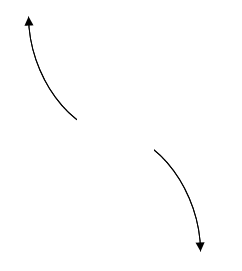
\includegraphics[width=0.3\textwidth]{../Figures/polyEndBehaviorCopyAA.png}
\end{center}\begin{enumerate}[label=\Alph*.]
\begin{multicols}{2}
\item 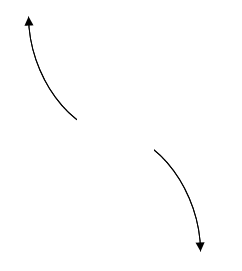
\includegraphics[width = 0.3\textwidth]{../Figures/polyEndBehaviorCopyAA.png}
\item 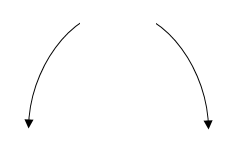
\includegraphics[width = 0.3\textwidth]{../Figures/polyEndBehaviorCopyBA.png}
\item 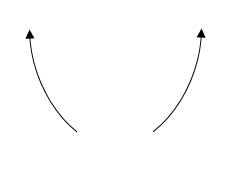
\includegraphics[width = 0.3\textwidth]{../Figures/polyEndBehaviorCopyCA.png}
\item 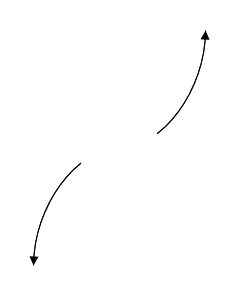
\includegraphics[width = 0.3\textwidth]{../Figures/polyEndBehaviorCopyDA.png}
\end{multicols}\item None of the above.\end{enumerate}
\textbf{General Comment:} Remember that end behavior is determined by the leading coefficient AND whether the \textbf{sum} of the multiplicities is positive or negative.
}
\litem{
Construct the lowest-degree polynomial given the zeros below. Then, choose the intervals that contain the coefficients of the polynomial in the form $ax^3+bx^2+cx+d$.
\[ \frac{-3}{2}, 3, \text{ and } \frac{2}{5} \]The solution is \( 10x^{3} -19 x^{2} -39 x + 18 \), which is option C.\begin{enumerate}[label=\Alph*.]
\item \( a \in [9, 13], b \in [-20, -16], c \in [-42, -33], \text{ and } d \in [-19, -12] \)

$10x^{3} -19 x^{2} -39 x -18$, which corresponds to multiplying everything correctly except the constant term.
\item \( a \in [9, 13], b \in [9, 17], c \in [-51, -46], \text{ and } d \in [13, 22] \)

$10x^{3} +11 x^{2} -51 x + 18$, which corresponds to multiplying out $(2x -3)(x + 3)(5x -2)$.
\item \( a \in [9, 13], b \in [-20, -16], c \in [-42, -33], \text{ and } d \in [13, 22] \)

* $10x^{3} -19 x^{2} -39 x + 18$, which is the correct option.
\item \( a \in [9, 13], b \in [-50, -48], c \in [63, 65], \text{ and } d \in [-19, -12] \)

$10x^{3} -49 x^{2} +63 x -18$, which corresponds to multiplying out $(2x -3)(x -3)(5x -2)$.
\item \( a \in [9, 13], b \in [19, 25], c \in [-42, -33], \text{ and } d \in [-19, -12] \)

$10x^{3} +19 x^{2} -39 x -18$, which corresponds to multiplying out $(2x -3)(x + 3)(5x + 2)$.
\end{enumerate}

\textbf{General Comment:} To construct the lowest-degree polynomial, you want to multiply out $(2x + 3)(x -3)(5x -2)$
}
\litem{
Describe the zero behavior of the zero $x = -8$ of the polynomial below.
\[ f(x) = -4(x + 8)^{5}(x - 8)^{10}(x + 2)^{8}(x - 2)^{12} \]The solution is the graph below, which is option A.
\begin{center}
    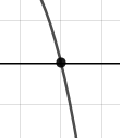
\includegraphics[width=0.3\textwidth]{../Figures/polyZeroBehaviorAA.png}
\end{center}\begin{enumerate}[label=\Alph*.]
\begin{multicols}{2}
\item 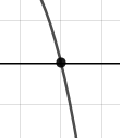
\includegraphics[width = 0.3\textwidth]{../Figures/polyZeroBehaviorAA.png}
\item 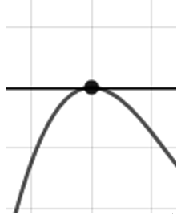
\includegraphics[width = 0.3\textwidth]{../Figures/polyZeroBehaviorBA.png}
\item 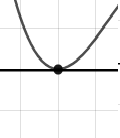
\includegraphics[width = 0.3\textwidth]{../Figures/polyZeroBehaviorCA.png}
\item 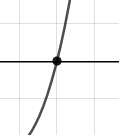
\includegraphics[width = 0.3\textwidth]{../Figures/polyZeroBehaviorDA.png}
\end{multicols}\item None of the above.\end{enumerate}
\textbf{General Comment:} You will need to sketch the entire graph, then zoom in on the zero the question asks about.
}
\litem{
Describe the end behavior of the polynomial below.
\[ f(x) = -2(x - 4)^{5}(x + 4)^{8}(x + 6)^{5}(x - 6)^{5} \]The solution is the graph below, which is option A.
\begin{center}
    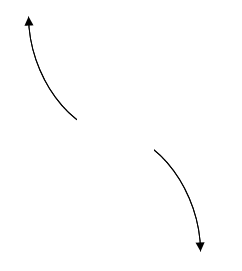
\includegraphics[width=0.3\textwidth]{../Figures/polyEndBehaviorAA.png}
\end{center}\begin{enumerate}[label=\Alph*.]
\begin{multicols}{2}
\item 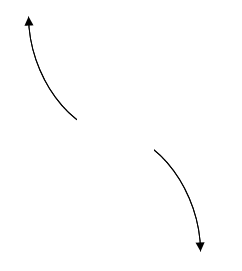
\includegraphics[width = 0.3\textwidth]{../Figures/polyEndBehaviorAA.png}
\item 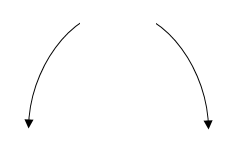
\includegraphics[width = 0.3\textwidth]{../Figures/polyEndBehaviorBA.png}
\item 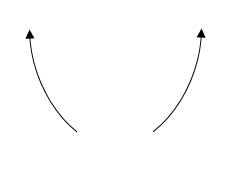
\includegraphics[width = 0.3\textwidth]{../Figures/polyEndBehaviorCA.png}
\item 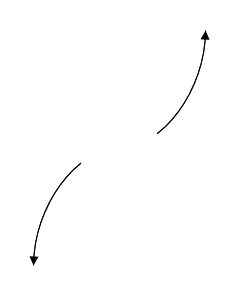
\includegraphics[width = 0.3\textwidth]{../Figures/polyEndBehaviorDA.png}
\end{multicols}\item None of the above.\end{enumerate}
\textbf{General Comment:} Remember that end behavior is determined by the leading coefficient AND whether the \textbf{sum} of the multiplicities is positive or negative.
}
\litem{
Construct the lowest-degree polynomial given the zeros below. Then, choose the intervals that contain the coefficients of the polynomial in the form $x^3+bx^2+cx+d$.
\[ 4 - 5 i \text{ and } 2 \]The solution is \( x^{3} -10 x^{2} +57 x -82 \), which is option B.\begin{enumerate}[label=\Alph*.]
\item \( b \in [-5, 5], c \in [-5, 4], \text{ and } d \in [-10, -7] \)

$x^{3} + x^{2} +3 x -10$, which corresponds to multiplying out $(x + 5)(x -2)$.
\item \( b \in [-11, -4], c \in [54, 62], \text{ and } d \in [-87, -81] \)

* $x^{3} -10 x^{2} +57 x -82$, which is the correct option.
\item \( b \in [-5, 5], c \in [-10, 1], \text{ and } d \in [7, 9] \)

$x^{3} + x^{2} -6 x + 8$, which corresponds to multiplying out $(x -4)(x -2)$.
\item \( b \in [9, 17], c \in [54, 62], \text{ and } d \in [79, 83] \)

$x^{3} +10 x^{2} +57 x + 82$, which corresponds to multiplying out $(x-(4 - 5 i))(x-(4 + 5 i))(x + 2)$.
\item \( \text{None of the above.} \)

This corresponds to making an unanticipated error or not understanding how to use nonreal complex numbers to create the lowest-degree polynomial. If you chose this and are not sure what you did wrong, please contact the coordinator for help.
\end{enumerate}

\textbf{General Comment:} Remember that the conjugate of $a+bi$ is $a-bi$. Since these zeros always come in pairs, we need to multiply out $(x-(4 - 5 i))(x-(4 + 5 i))(x-(2))$.
}
\litem{
Which of the following equations \textit{could} be of the graph presented below?

\begin{center}
    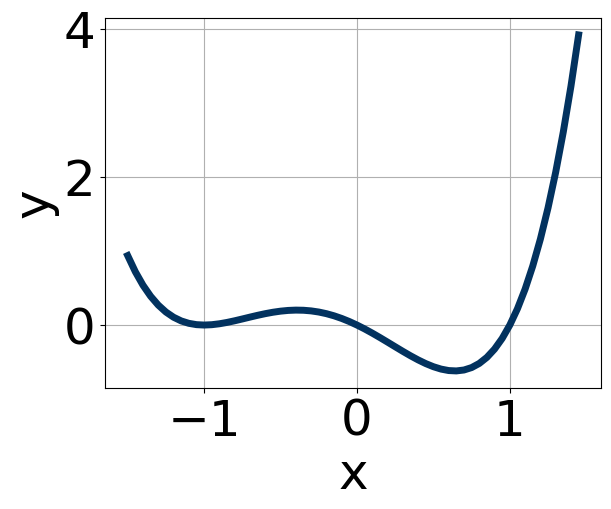
\includegraphics[width=0.5\textwidth]{../Figures/polyGraphToFunctionA.png}
\end{center}


The solution is \( 13x^{11} (x - 1)^{11} (x + 2)^{9} \), which is option C.\begin{enumerate}[label=\Alph*.]
\item \( -13x^{11} (x - 1)^{7} (x + 2)^{5} \)

This corresponds to the leading coefficient being the opposite value than it should be.
\item \( 13x^{9} (x - 1)^{8} (x + 2)^{9} \)

The factor $1$ should have been an odd power.
\item \( 13x^{11} (x - 1)^{11} (x + 2)^{9} \)

* This is the correct option.
\item \( -18x^{7} (x - 1)^{8} (x + 2)^{7} \)

The factor $(x - 1)$ should have an odd power and the leading coefficient should be the opposite sign.
\item \( 18x^{4} (x - 1)^{10} (x + 2)^{11} \)

The factors $1$ and $0$ have have been odd power.
\end{enumerate}

\textbf{General Comment:} General Comments: Draw the x-axis to determine which zeros are touching (and so have even multiplicity) or cross (and have odd multiplicity).
}
\litem{
Construct the lowest-degree polynomial given the zeros below. Then, choose the intervals that contain the coefficients of the polynomial in the form $x^3+bx^2+cx+d$.
\[ -3 + 5 i \text{ and } 4 \]The solution is \( x^{3} +2 x^{2} +10 x -136 \), which is option C.\begin{enumerate}[label=\Alph*.]
\item \( b \in [-4.9, -0.1], c \in [9, 18], \text{ and } d \in [134, 142] \)

$x^{3} -2 x^{2} +10 x + 136$, which corresponds to multiplying out $(x-(-3 + 5 i))(x-(-3 - 5 i))(x + 4)$.
\item \( b \in [-0.2, 1.3], c \in [-1, 9], \text{ and } d \in [-14, -5] \)

$x^{3} + x^{2} -x -12$, which corresponds to multiplying out $(x + 3)(x -4)$.
\item \( b \in [1.2, 8], c \in [9, 18], \text{ and } d \in [-137, -135] \)

* $x^{3} +2 x^{2} +10 x -136$, which is the correct option.
\item \( b \in [-0.2, 1.3], c \in [-14, -8], \text{ and } d \in [20, 25] \)

$x^{3} + x^{2} -9 x + 20$, which corresponds to multiplying out $(x -5)(x -4)$.
\item \( \text{None of the above.} \)

This corresponds to making an unanticipated error or not understanding how to use nonreal complex numbers to create the lowest-degree polynomial. If you chose this and are not sure what you did wrong, please contact the coordinator for help.
\end{enumerate}

\textbf{General Comment:} Remember that the conjugate of $a+bi$ is $a-bi$. Since these zeros always come in pairs, we need to multiply out $(x-(-3 + 5 i))(x-(-3 - 5 i))(x-(4))$.
}
\litem{
Describe the zero behavior of the zero $x = -3$ of the polynomial below.
\[ f(x) = -9(x - 3)^{4}(x + 3)^{5}(x - 8)^{4}(x + 8)^{8} \]The solution is the graph below, which is option A.
\begin{center}
    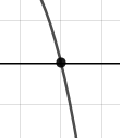
\includegraphics[width=0.3\textwidth]{../Figures/polyZeroBehaviorCopyAA.png}
\end{center}\begin{enumerate}[label=\Alph*.]
\begin{multicols}{2}
\item 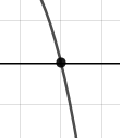
\includegraphics[width = 0.3\textwidth]{../Figures/polyZeroBehaviorCopyAA.png}
\item 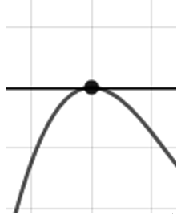
\includegraphics[width = 0.3\textwidth]{../Figures/polyZeroBehaviorCopyBA.png}
\item 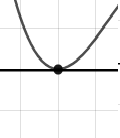
\includegraphics[width = 0.3\textwidth]{../Figures/polyZeroBehaviorCopyCA.png}
\item 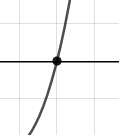
\includegraphics[width = 0.3\textwidth]{../Figures/polyZeroBehaviorCopyDA.png}
\end{multicols}\item None of the above.\end{enumerate}
\textbf{General Comment:} You will need to sketch the entire graph, then zoom in on the zero the question asks about.
}
\litem{
Construct the lowest-degree polynomial given the zeros below. Then, choose the intervals that contain the coefficients of the polynomial in the form $ax^3+bx^2+cx+d$.
\[ \frac{5}{4}, \frac{-1}{3}, \text{ and } \frac{-7}{3} \]The solution is \( 36x^{3} +51 x^{2} -92 x -35 \), which is option C.\begin{enumerate}[label=\Alph*.]
\item \( a \in [31, 37], b \in [51, 53], c \in [-96, -85], \text{ and } d \in [27, 44] \)

$36x^{3} +51 x^{2} -92 x + 35$, which corresponds to multiplying everything correctly except the constant term.
\item \( a \in [31, 37], b \in [-55, -44], c \in [-96, -85], \text{ and } d \in [27, 44] \)

$36x^{3} -51 x^{2} -92 x + 35$, which corresponds to multiplying out $(4x + 5)(3x -1)(3x -7)$.
\item \( a \in [31, 37], b \in [51, 53], c \in [-96, -85], \text{ and } d \in [-41, -27] \)

* $36x^{3} +51 x^{2} -92 x -35$, which is the correct option.
\item \( a \in [31, 37], b \in [117, 121], c \in [62, 71], \text{ and } d \in [-41, -27] \)

$36x^{3} +117 x^{2} +62 x -35$, which corresponds to multiplying out $(4x + 5)(3x -1)(3x + 7)$.
\item \( a \in [31, 37], b \in [140, 143], c \in [142, 157], \text{ and } d \in [27, 44] \)

$36x^{3} +141 x^{2} +148 x + 35$, which corresponds to multiplying out $(4x + 5)(3x + 1)(3x + 7)$.
\end{enumerate}

\textbf{General Comment:} To construct the lowest-degree polynomial, you want to multiply out $(4x -5)(3x + 1)(3x + 7)$
}
\end{enumerate}

\end{document}